\chapter{Design}

The HaptiQ aims to solve some of the problems identifies in the related work. The hardware was developed using an iterative explorative process. Therefore the design phases largely overlap with the implementation ones. The API provided has also undergone through many iterations. In this chapter I will first discuss the earliest prototypes. Then the 4-HaptiQ and the 8-HaptiQ hardware designs are illustrated. Finally, a detailed overview of the API is provided.

\section{The Hardware}
\subsection{Early Prototypes}
The hardware design of the HaptiQ has been initially based on the HTP design. Similarly to the HTP, the HaptiQ also uses mini-servos to control its actuators. However, while the HTP controls only one actuator, the HaptiQ controls four or eight of them. It immediately follows that as the number of actuators increases, so do the number of servos and the size of the device. In order to minimise the size I designed three main prototypes by sketches (see Figure ~\ref{fig:HaptiQ-early-prototypes}). 

The first prototype extends the rotational axis in the xy plane (see Figure ~\ref{fig:first prototype}). The extension is designed as a gear that allows to choose combinations of three aligned actuators. An additional actuator would then be used to raise the selected actuators. This design reduces the number of servos, but all raised actuators will have the same height. Note that the focus of this design sketch was to minimise the number of servos, that is why actuators are shown as points, similar to Braille displays.

\begin{figure}
        \centering
        \begin{subfigure}[H]{0.5\textwidth}
                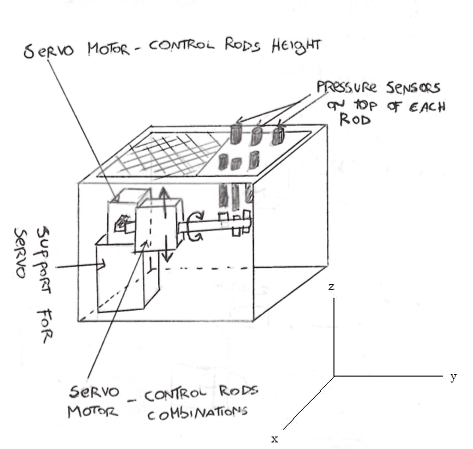
\includegraphics[width=\textwidth,height=\textwidth]{prototype1.png}
                \caption{Grid based}
                \label{fig:first prototype}
        \end{subfigure}%
        ~ %add desired spacing between images, e. g. ~, \quad, \qquad etc.
          %(or a blank line to force the subfigure onto a new line)
        \begin{subfigure}[H]{0.5\textwidth}
                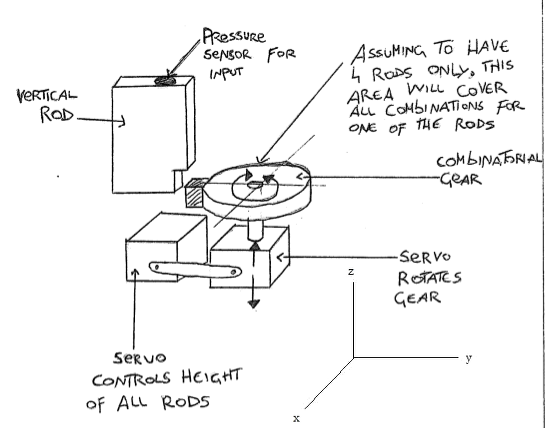
\includegraphics[width=\textwidth,height=\textwidth]{prototype2.png}
                \caption{Gear based}
                \label{fig:second prototype}
        \end{subfigure}
        ~ %add desired spacing between images, e. g. ~, \quad, \qquad etc.
          %(or a blank line to force the subfigure onto a new line)
        \begin{subfigure}[H]{0.5\textwidth}
                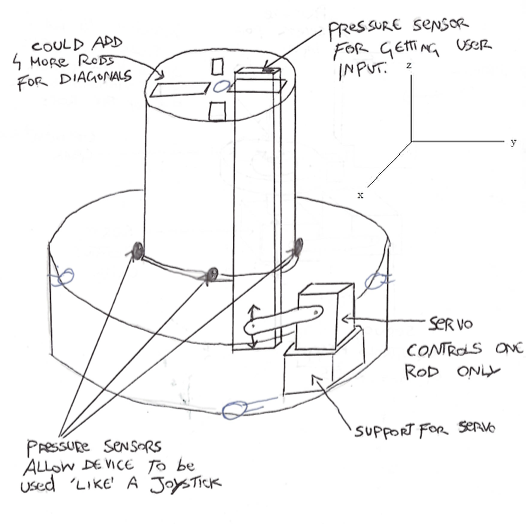
\includegraphics[width=\textwidth,height=\textwidth]{prototype3.png}
                \caption{One servo per actuator}
                \label{fig:third prototype}
        \end{subfigure}
        \caption{HaptiQ early prototypes}\label{fig:HaptiQ-early-prototypes}
\end{figure}

In the second prototype I tried to minimize the total number of servos to two. One servo would be used to rotate a combinatorial gear about the z-axis(see Figure ~\ref{fig:second prototype}). A second servo can then be used to raise the first servo with the gear it controls and all the rods. This approach can be consired very versatile and could allow an high number of actuators by keeping the number of servos always to two. Nonetheless, the actuators would all be at the same heights when raised as in the first prototype. Since height can be used to convey additional information, this prototype was discarded and a third prototype was created.

The third prototype does not focus on minimising the number of servos anymore, but rather on the possible functionalities that could be added to the HaptiQ. In this design each servo controls an actuator only and these are disposed circularly around the center of the device (see Figure ~\ref{fig:third prototype}). The device would have a "joystick" shape. Three pressure sensors could be added either at the bottom of the device or in between the internal and the external annuli. Using simple triangulation on the pressure sensors values, it could be possible to use the device like a gaming joystick and eventually augment its area of interaction. However, in one of the meetings with Saad, we realised that blind people would find this feature disrupting because understanding how far in the xy plane the device is augmented can become a challenging task. 

\subsection{4-HaptiQ}
The 4-HaptiQ is the first functional HaptiQ. This is an experimental project, with future work discussed in chapter 9, so I will occasionally refer to the device with the term prototype. This version has four actuators as shown in figure ~\ref{fig:HaptiQ reference static actuators}. Unlike the third of the early prototypes, the main focus is on the mechanics and functionalities aspects.
The most successful aspect of the HTP, most probably, is the use of a small servo to mechanically move the rod along the z-axis. Nonetheless, the mechanic design used in the HTP has some flows that the HaptiQ tries to solve. The HTP, in fact, transforms the rotational motion of the servo to a linear motion only by ensuring that the servo works under a small range and that the rod slices outside the device through a small opening.
In the HaptiQ the actuators slide through a guide that allows motion only in the z-direction. In addition, each servo is linked to its actuator by using one or more screws inserted in between small openings in the actuator (see Figures ~\ref{fig:HaptiQ MinPos} and ~\ref{fig:HaptiQ MaxPos}). 

\begin{figure}
        \centering
        \begin{subfigure}[H]{0.3\textwidth}
                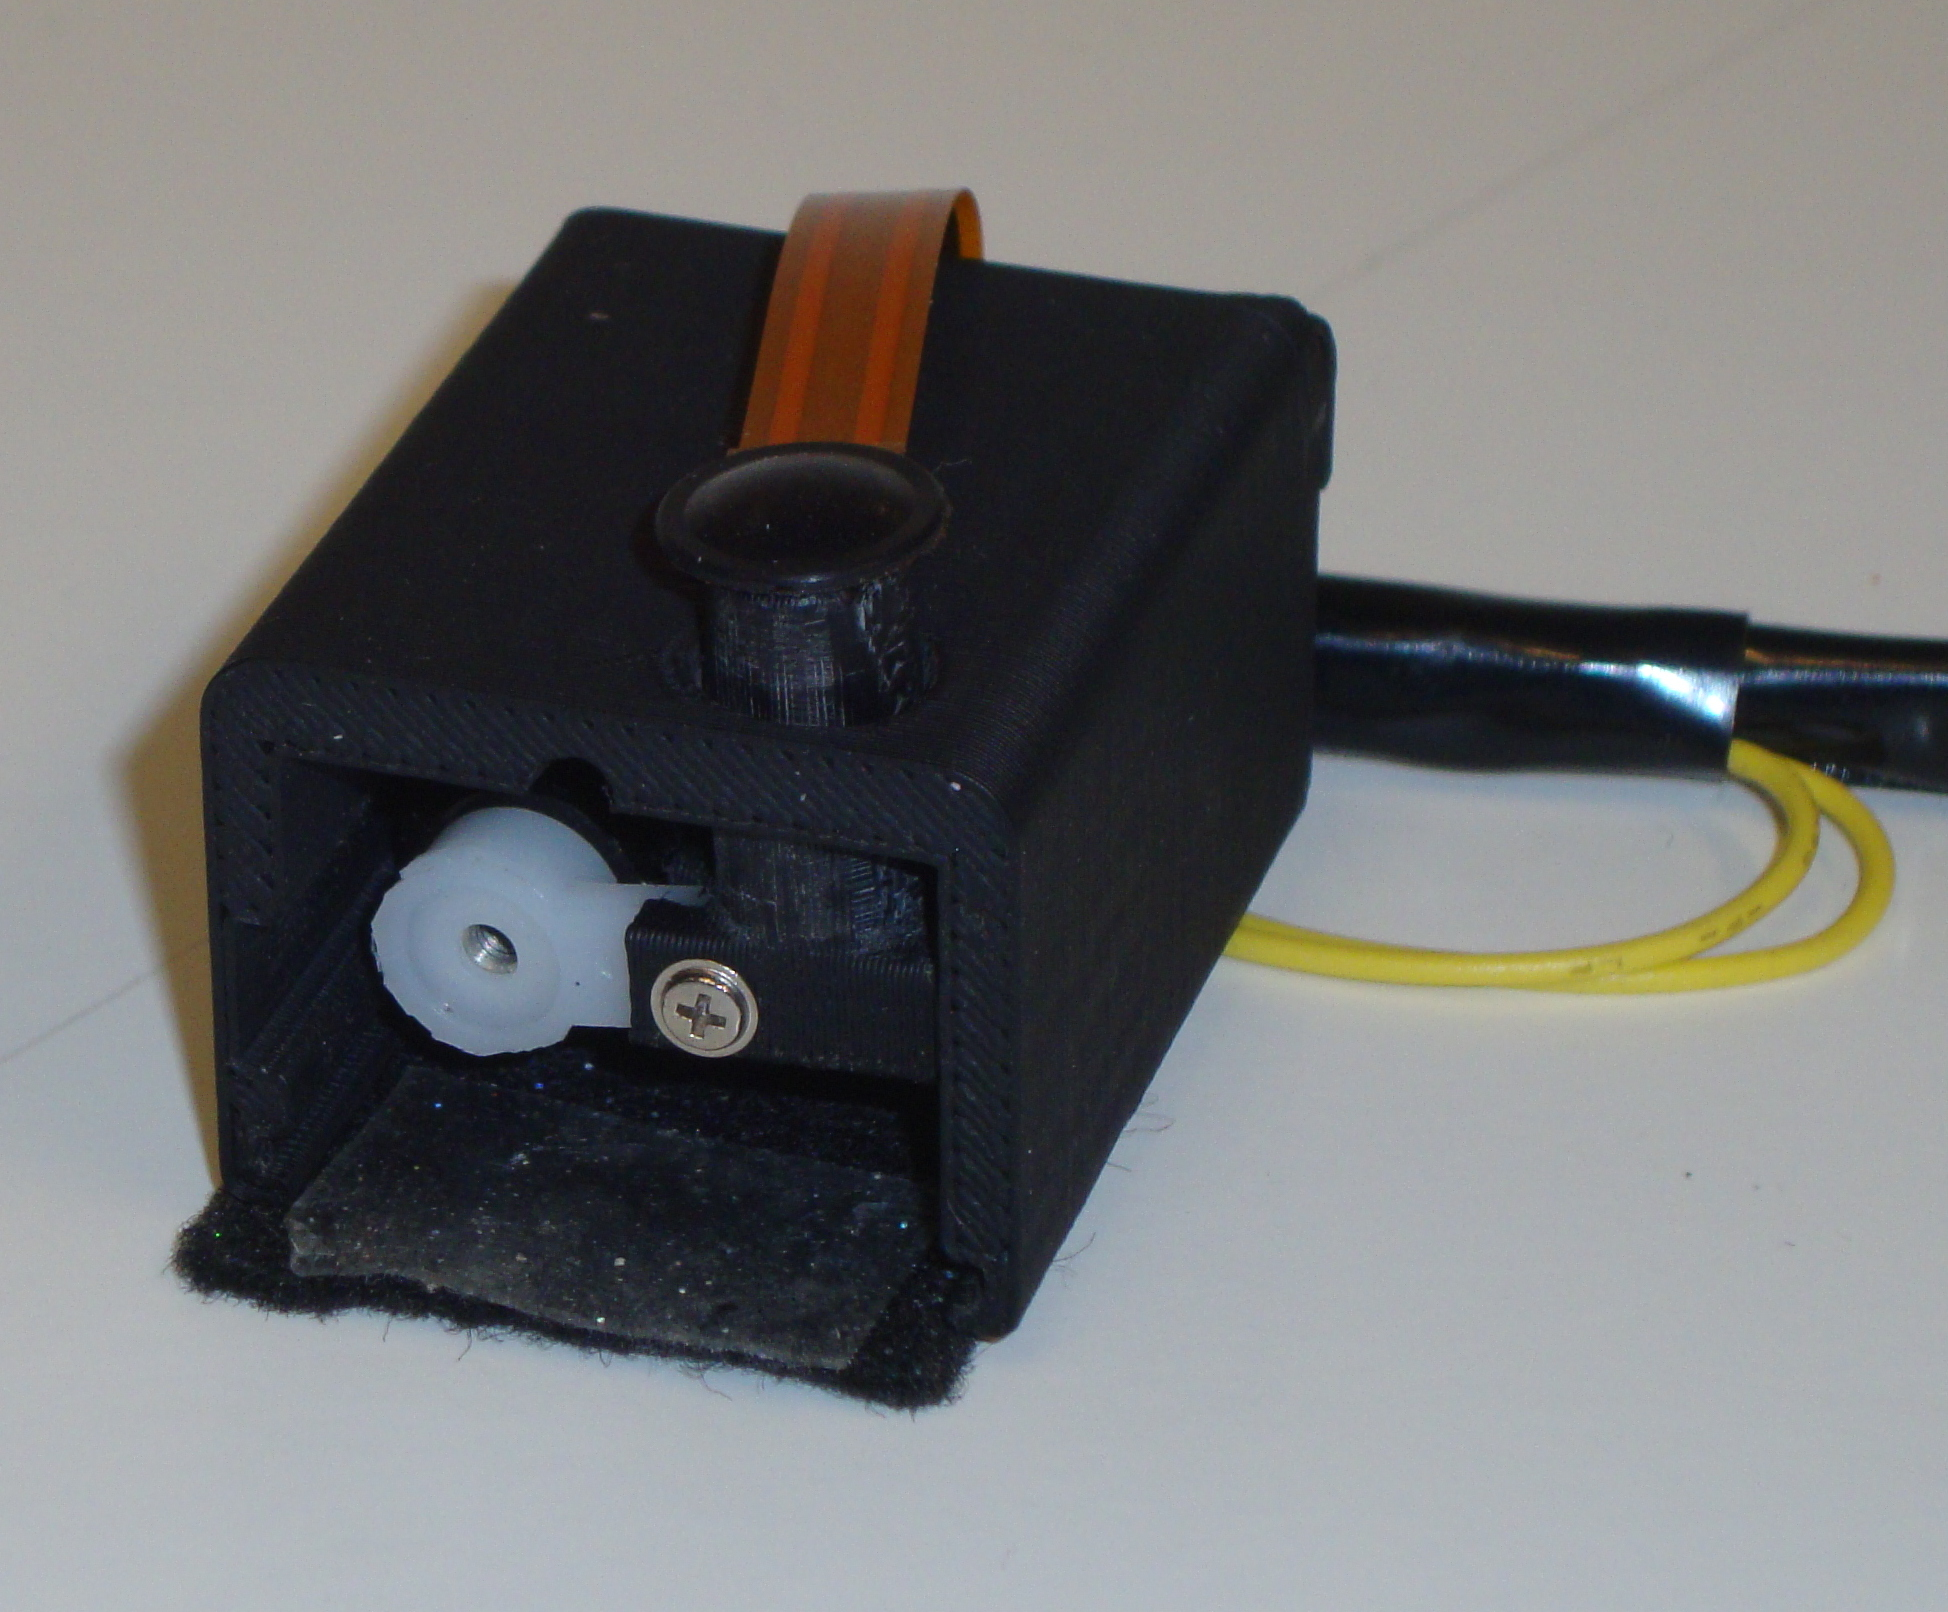
\includegraphics[width=\textwidth,height=\textwidth]{htp2.JPG}
                \caption{HTP}
                \label{fig:Mechanics HTP}
        \end{subfigure}%
        ~ %add desired spacing between images, e. g. ~, \quad, \qquad etc.
          %(or a blank line to force the subfigure onto a new line)
        \begin{subfigure}[H]{0.3\textwidth}
                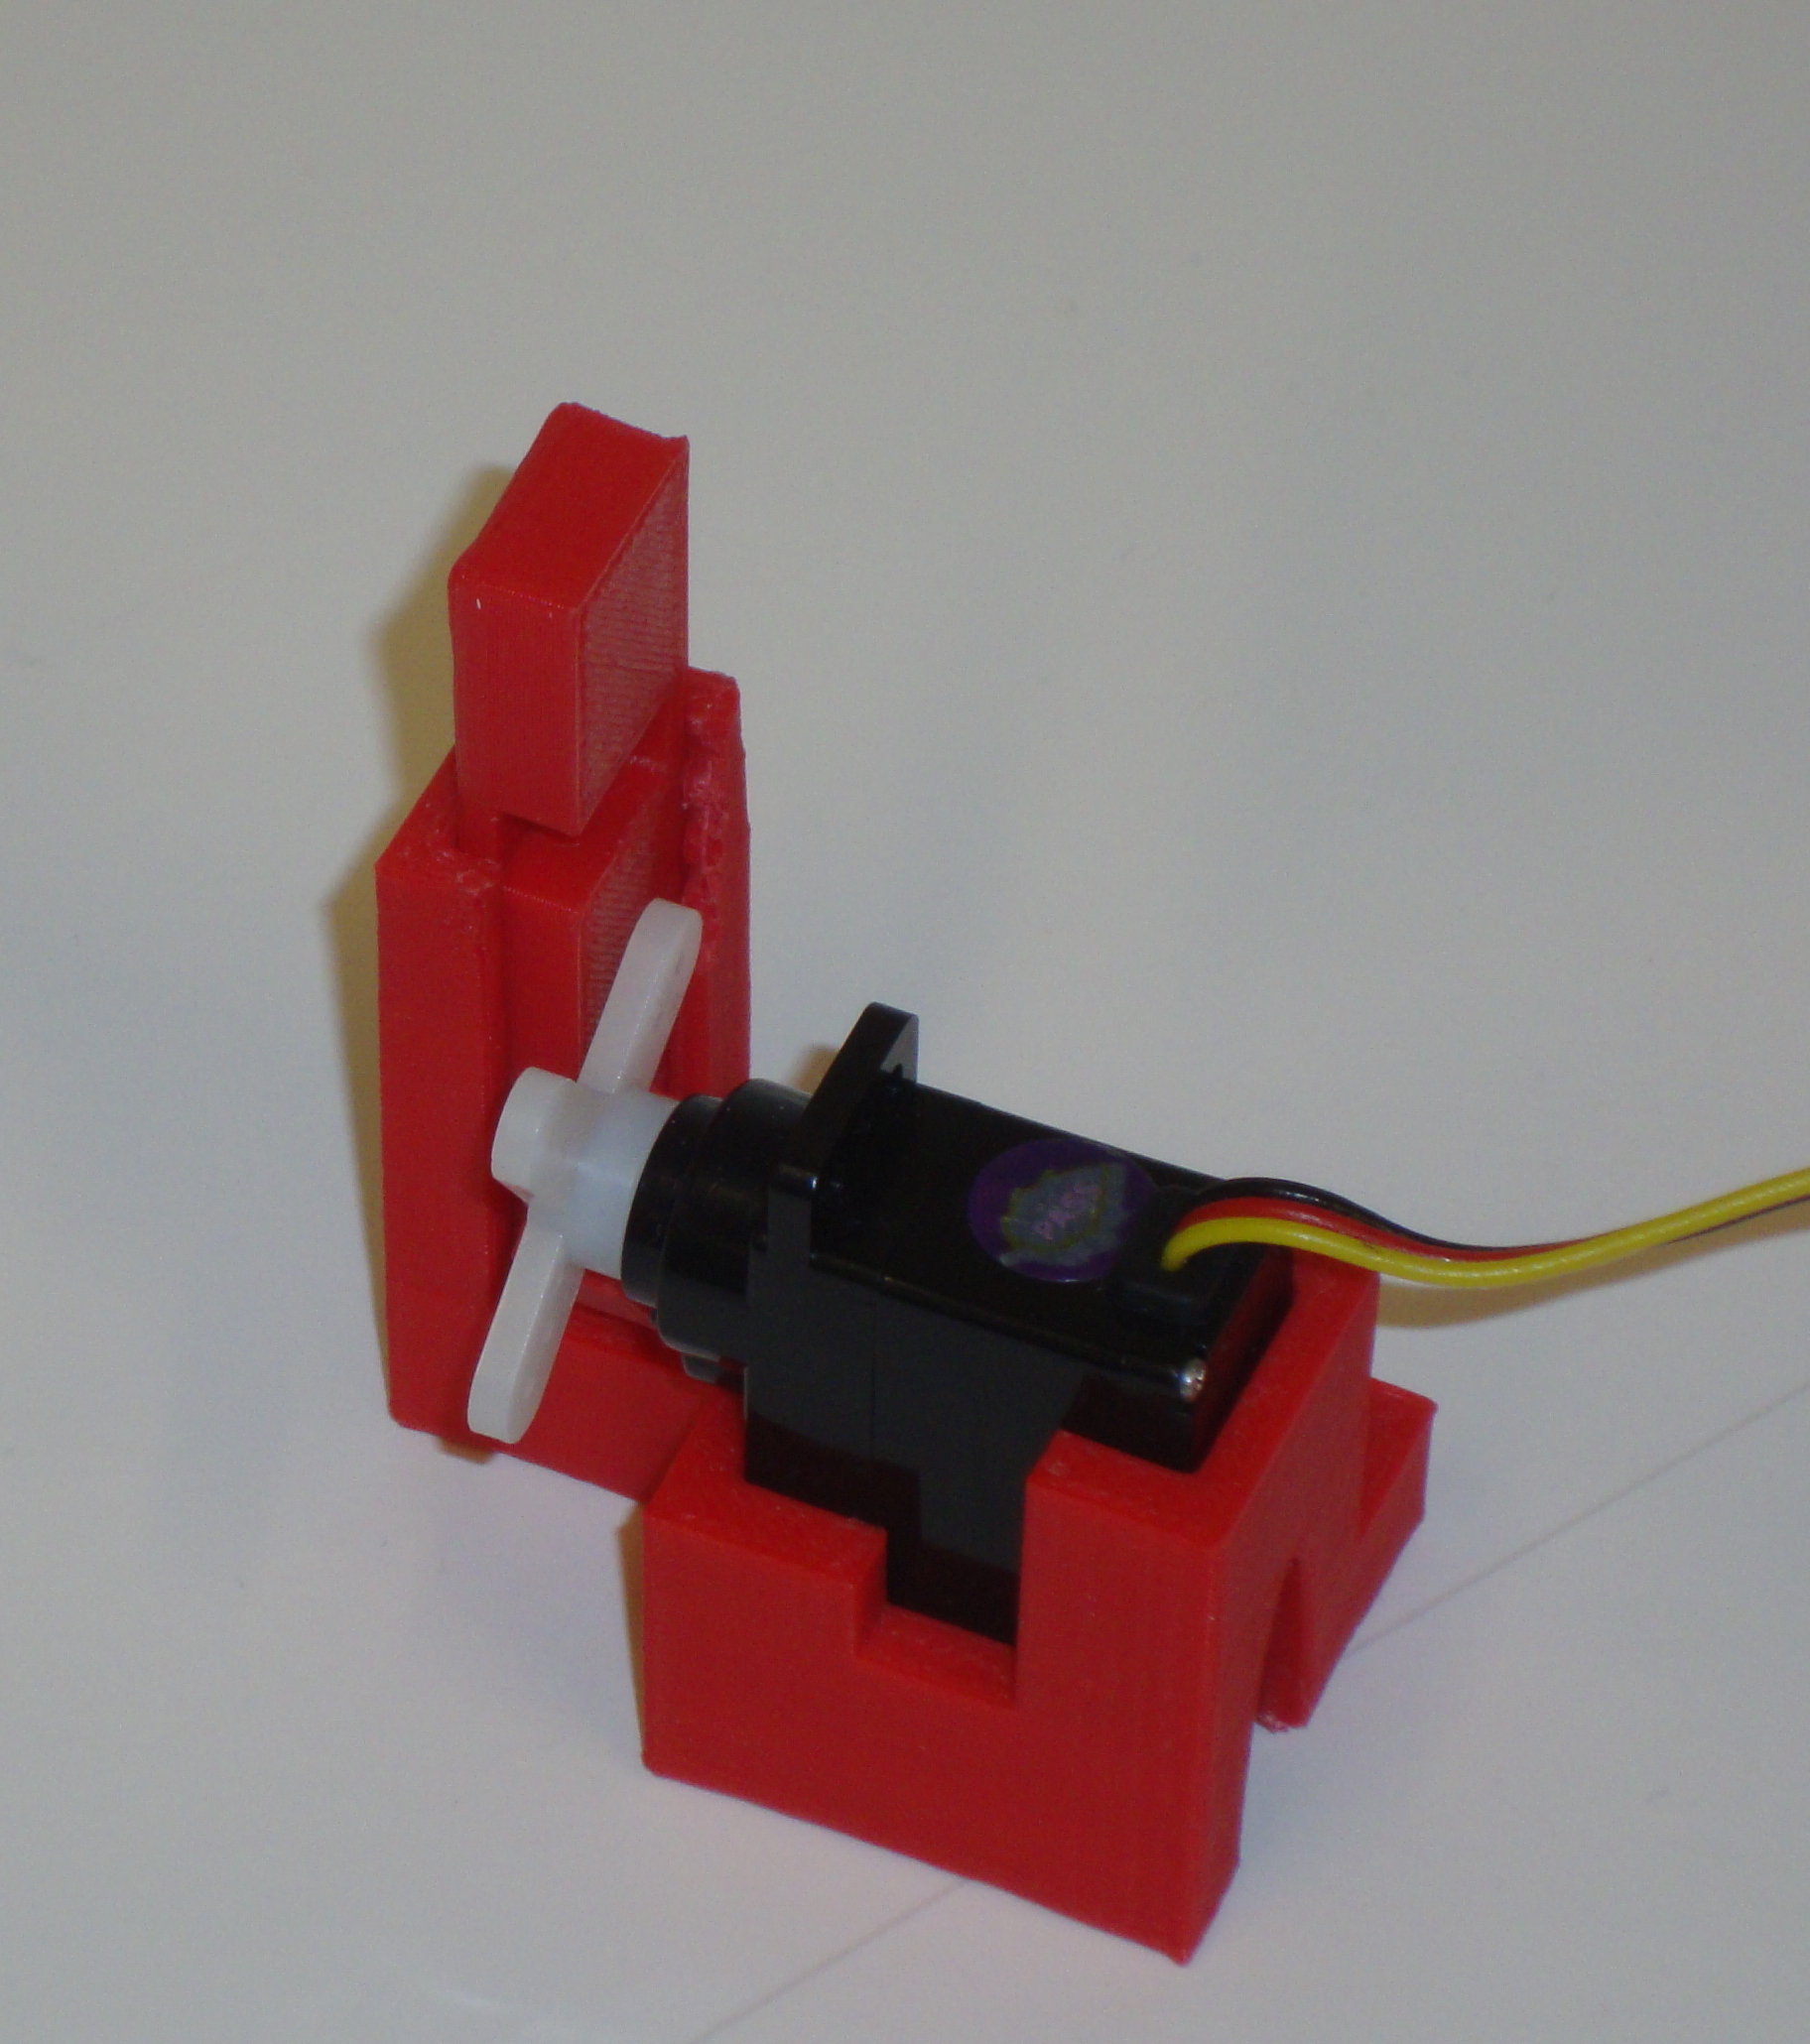
\includegraphics[width=\textwidth,height=\textwidth]{pos1.JPG}
                \caption{HaptiQ MinPos}
                \label{fig:HaptiQ MinPos}
        \end{subfigure}
        ~ %add desired spacing between images, e. g. ~, \quad, \qquad etc.
          %(or a blank line to force the subfigure onto a new line)
        \begin{subfigure}[H]{0.3\textwidth}
                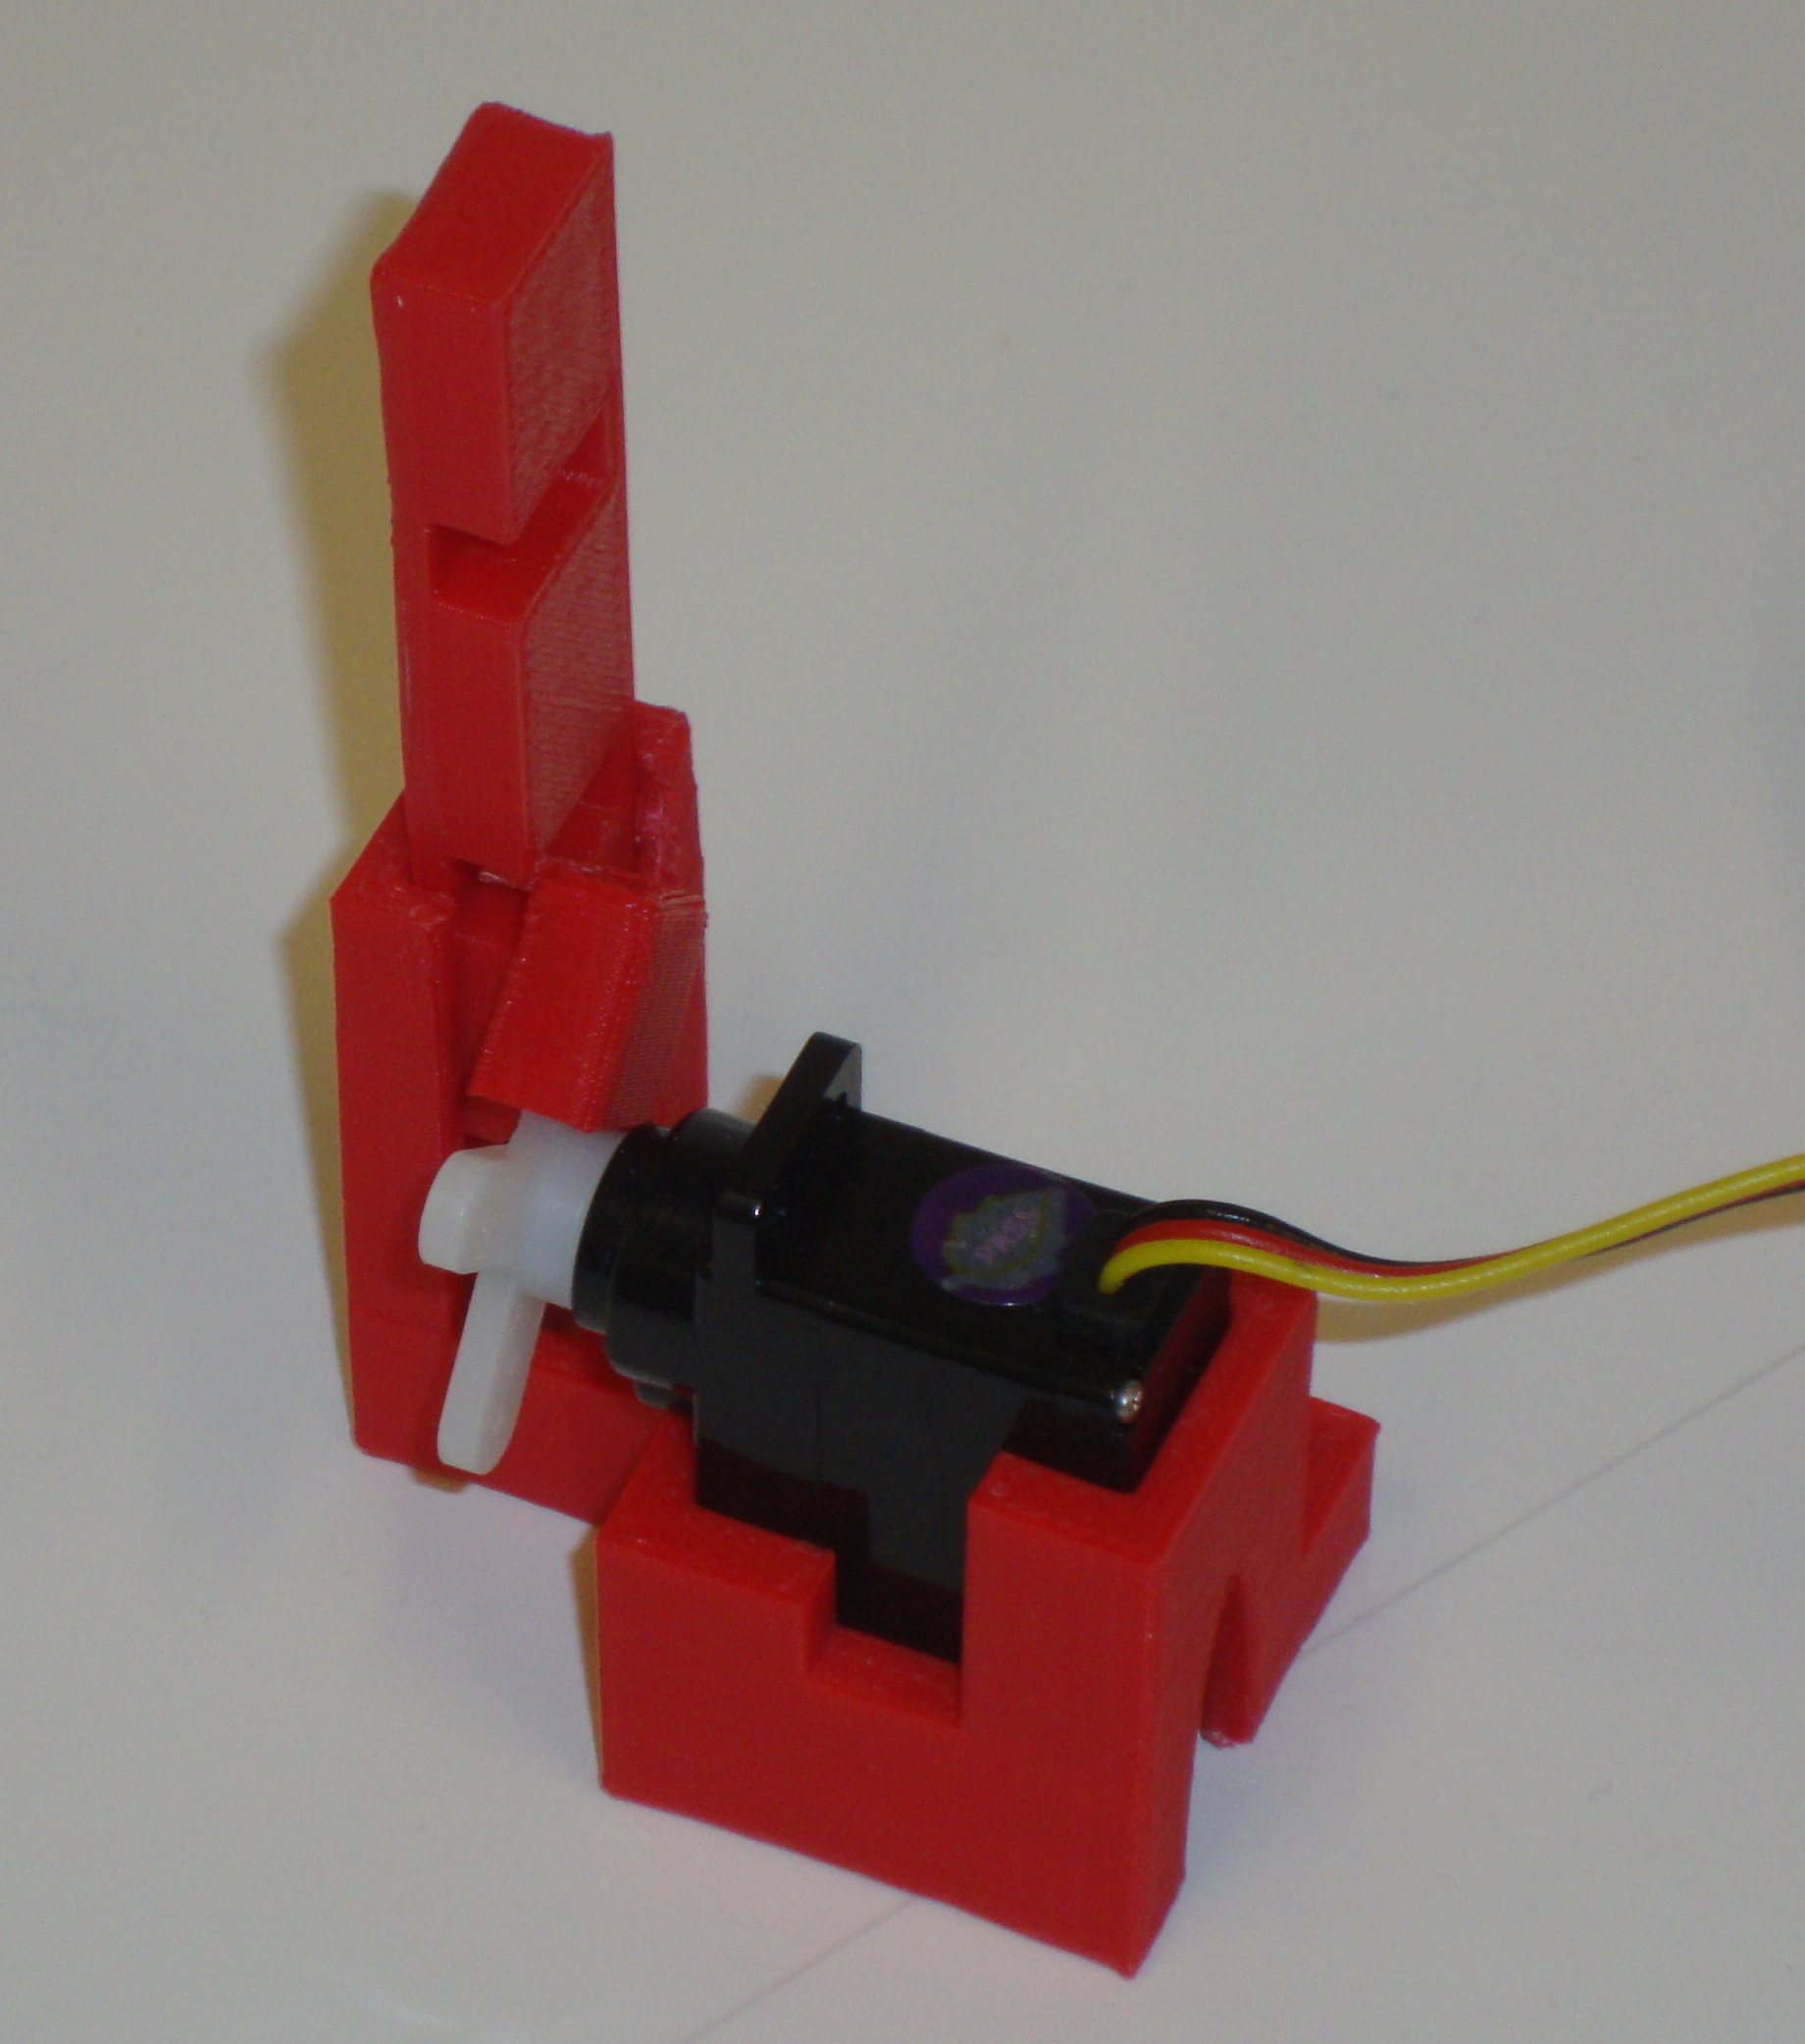
\includegraphics[width=\textwidth,height=\textwidth]{pos2.JPG}
                \caption{HaptiQ MaxPos}
                \label{fig:HaptiQ MaxPos}
        \end{subfigure}
        \caption{HTP and HaptiQ actuator mechanics}\label{fig:HTP and HaptiQ actuator mechanics}
\end{figure}

This version of the HaptiQ does not provide any case. The uneven surface leads to the lack of a reference point or plane for the actuators. This is a major problem in cases where the actuators change position while the user is not currently laying his hand on the device. In fact, it follows that when the blind user places the hand on top of the device again, he or her is not able to tell what the current state of the actuators is compared to the previous one. Two solutions are provided for the 4-HaptiQ: a mid-point reference and a plane reference static actuators (see Figure ~\ref{fig:HaptiQ reference static actuators}). It is not clear which type of reference actuator works best though. My hypothesis is that the plane reference actuator should be more comfortable when using the device and provides the same functionality than the point reference actuator. 

\begin{figure}
        \centering
        \begin{subfigure}[H]{0.5\textwidth}
                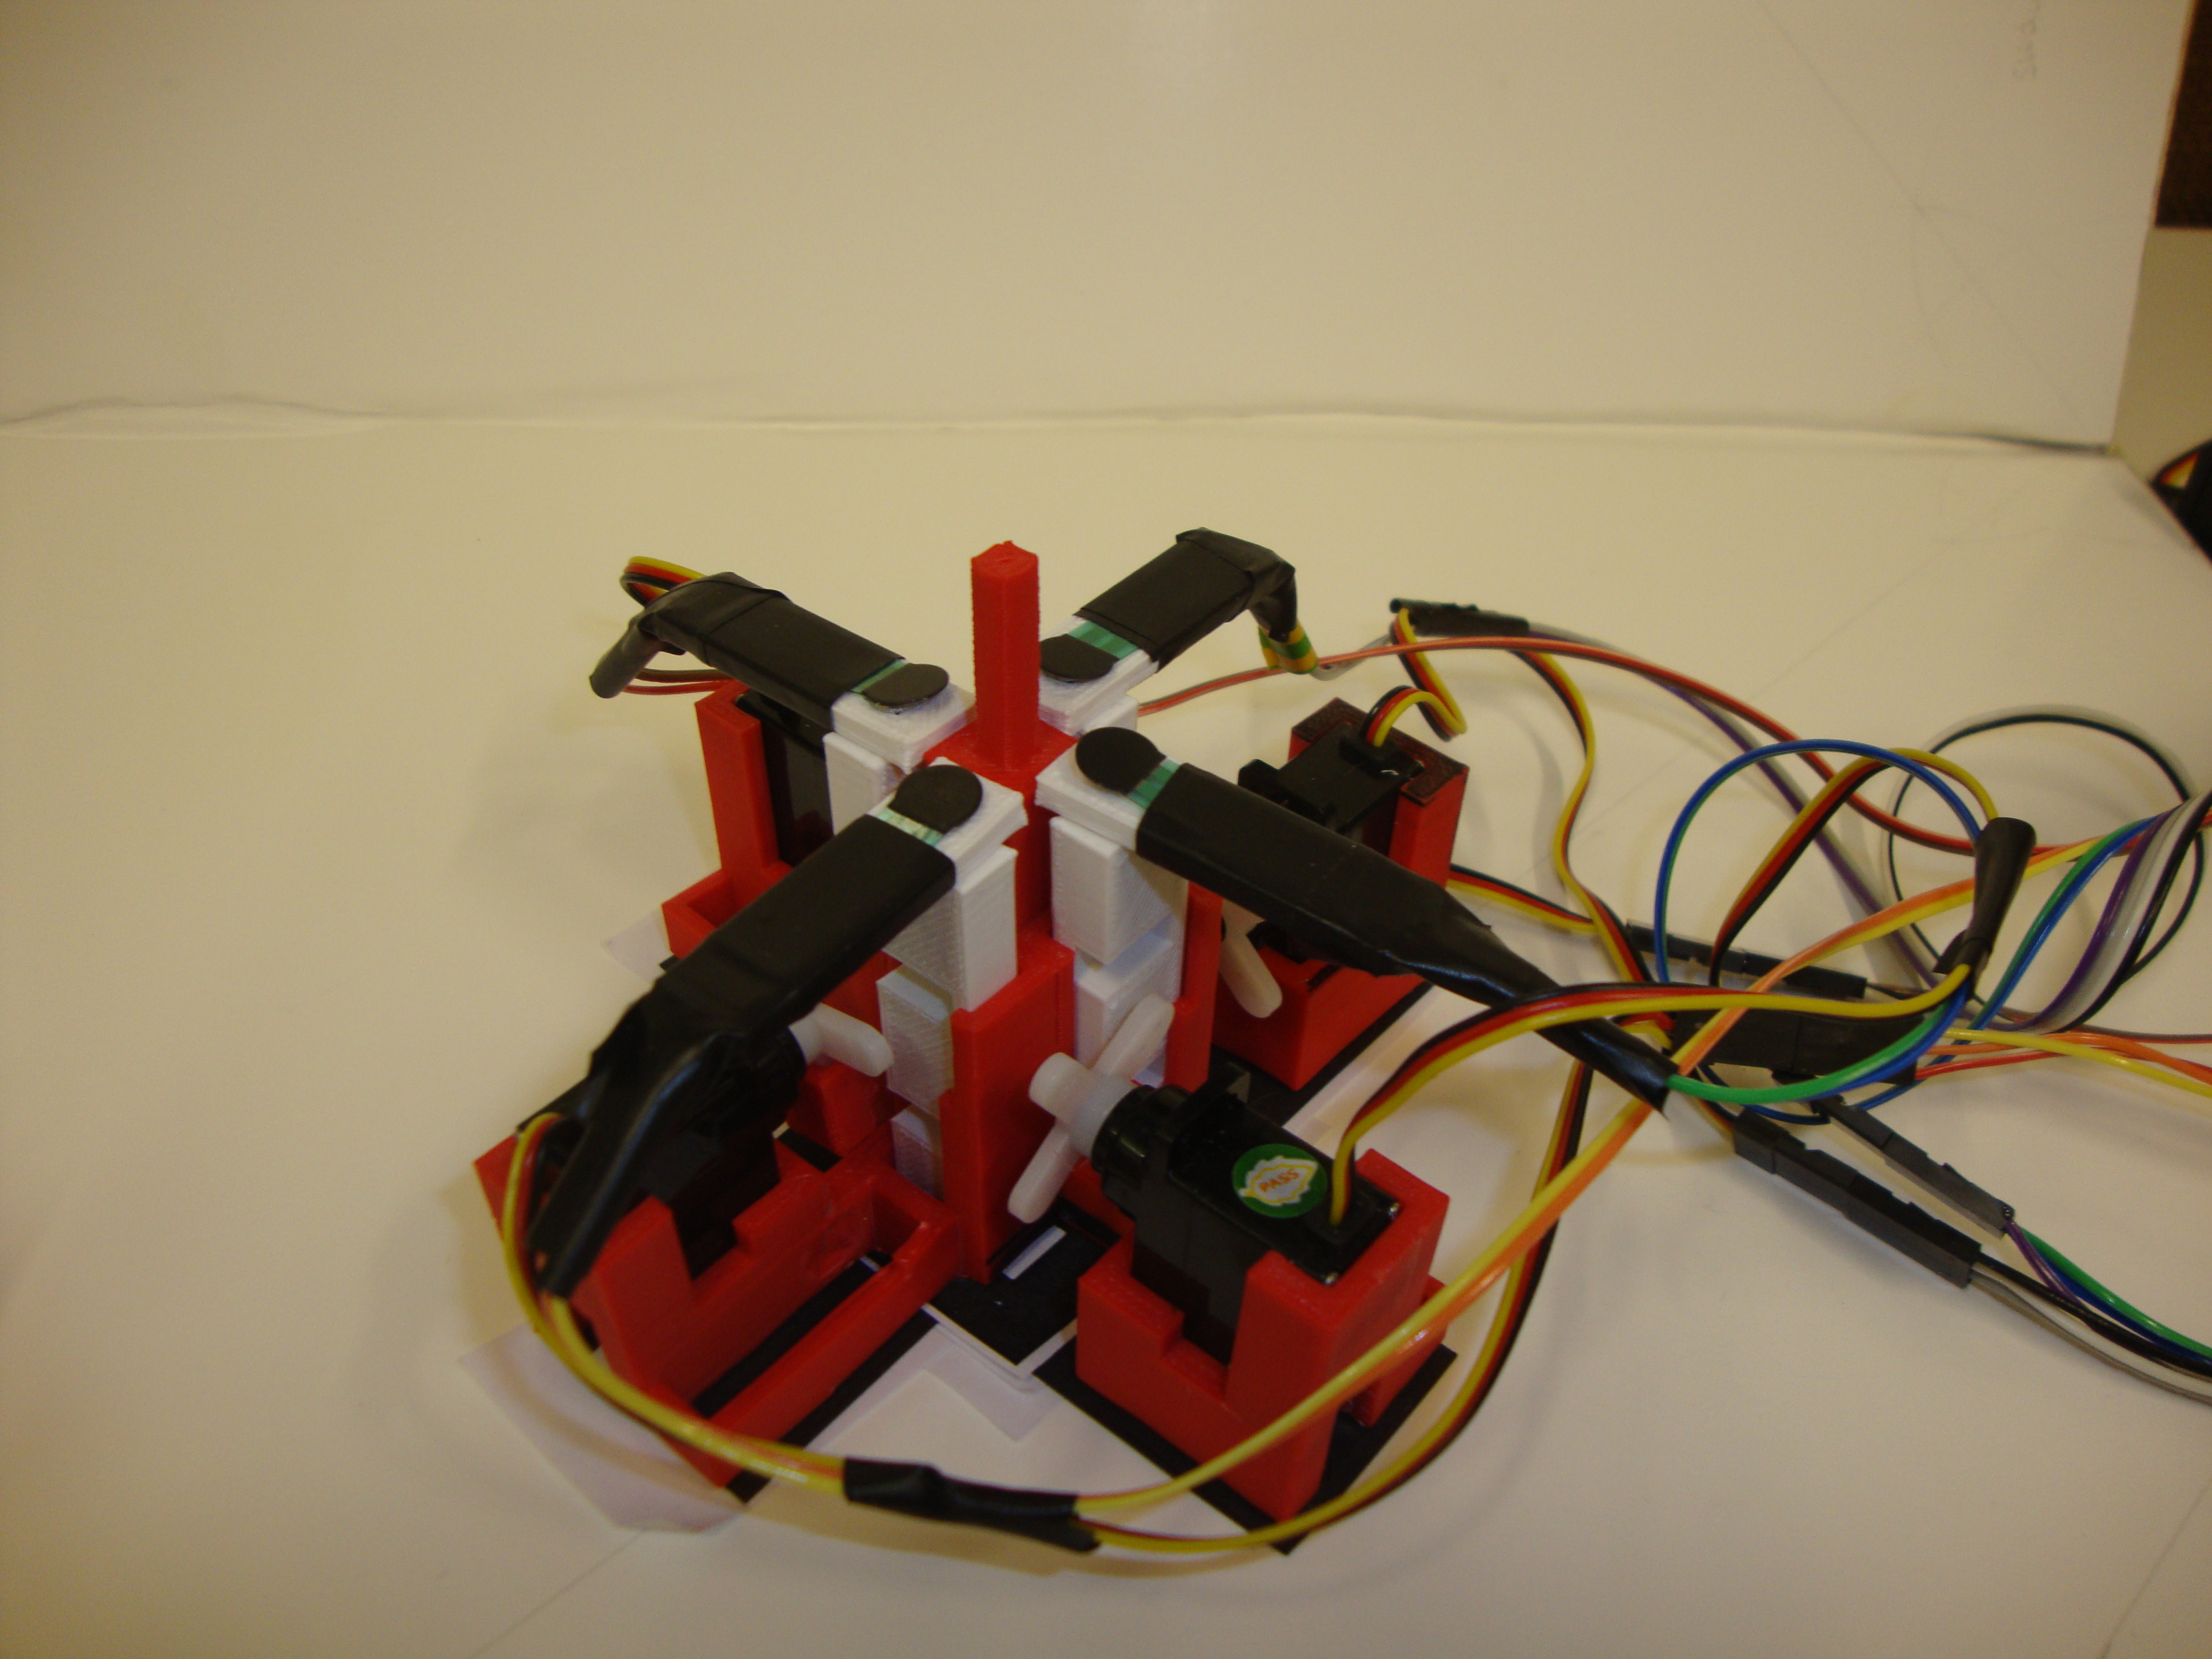
\includegraphics[width=\textwidth]{referencetype20.JPG}
                \caption{Mid-Point reference actuator}
                \label{fig:Mid-Point reference actuator}
        \end{subfigure}%
        ~ %add desired spacing between images, e. g. ~, \quad, \qquad etc.
          %(or a blank line to force the subfigure onto a new line)
        \begin{subfigure}[H]{0.5\textwidth}
                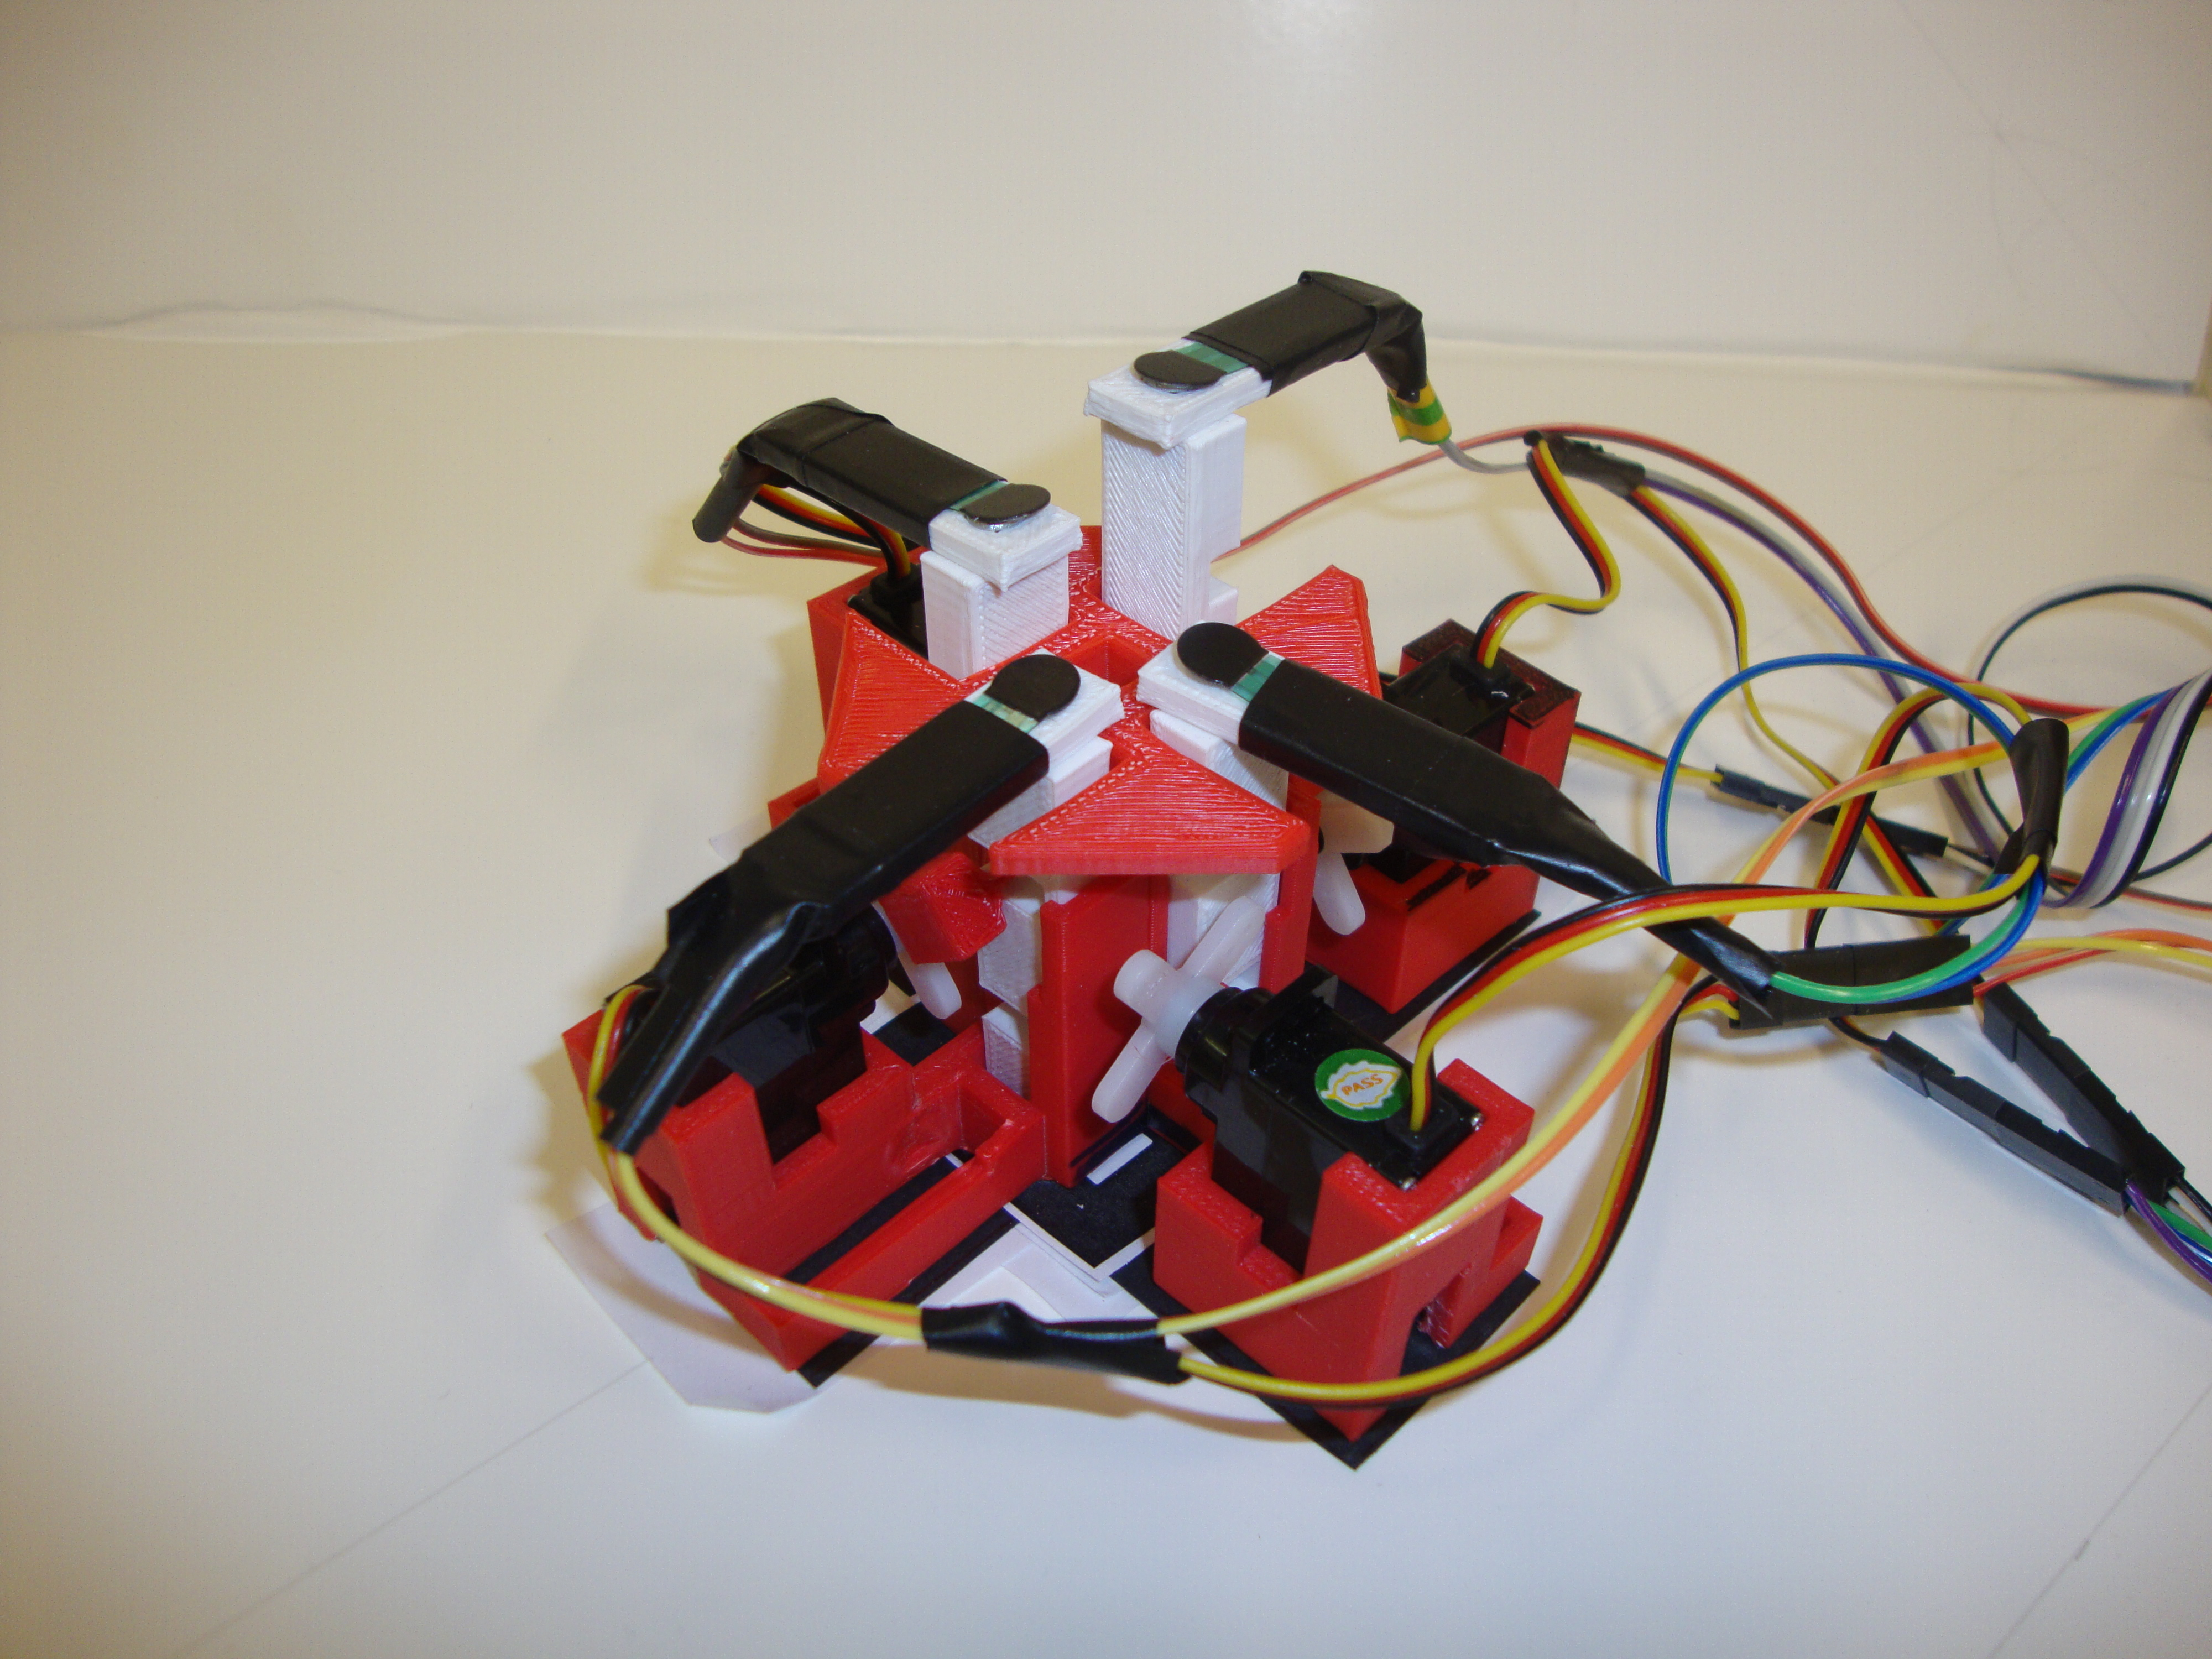
\includegraphics[width=\textwidth]{referencetype11.JPG}
                \caption{Plane reference actuator}
                \label{fig:Plane reference actuator}
        \end{subfigure}
        ~ %add desired spacing between images, e. g. ~, \quad, \qquad etc.
        \caption{HaptiQ reference static actuators}\label{fig:HaptiQ reference static actuators}
\end{figure}

The HaptiQ is the first vector-based display for blind users. Whether this design provides better feedback to users or not is unknown, because no study with participants could be conducted. Therefore, the actuators are designed so to support different tops in order to be able to evaluate the HaptiQ against a point-based haptic feedback TUI. In the version here presented, only vector-like tops are provided, but other type of tops can be easily printed and fasten to the actuators.   

Finally, the HaptiQ does not have any break to simulate friction. While it could be possible to add this feature, I decided that the primary goal of this project was just to focus on the vectorisation of the actuators. 

\subsection{8-HaptiQ}
The result of the final design iteration is the 8-HaptiQ. Using the same design of the 4-HaptiQ for eight actuators would lead to a considerable increase in size of the device. Therefore, the 8-HaptiQ has been completely re-engineered (see Figure ~\ref{fig:8-HaptiQ}). 

\begin{figure}[H]
  \centering
  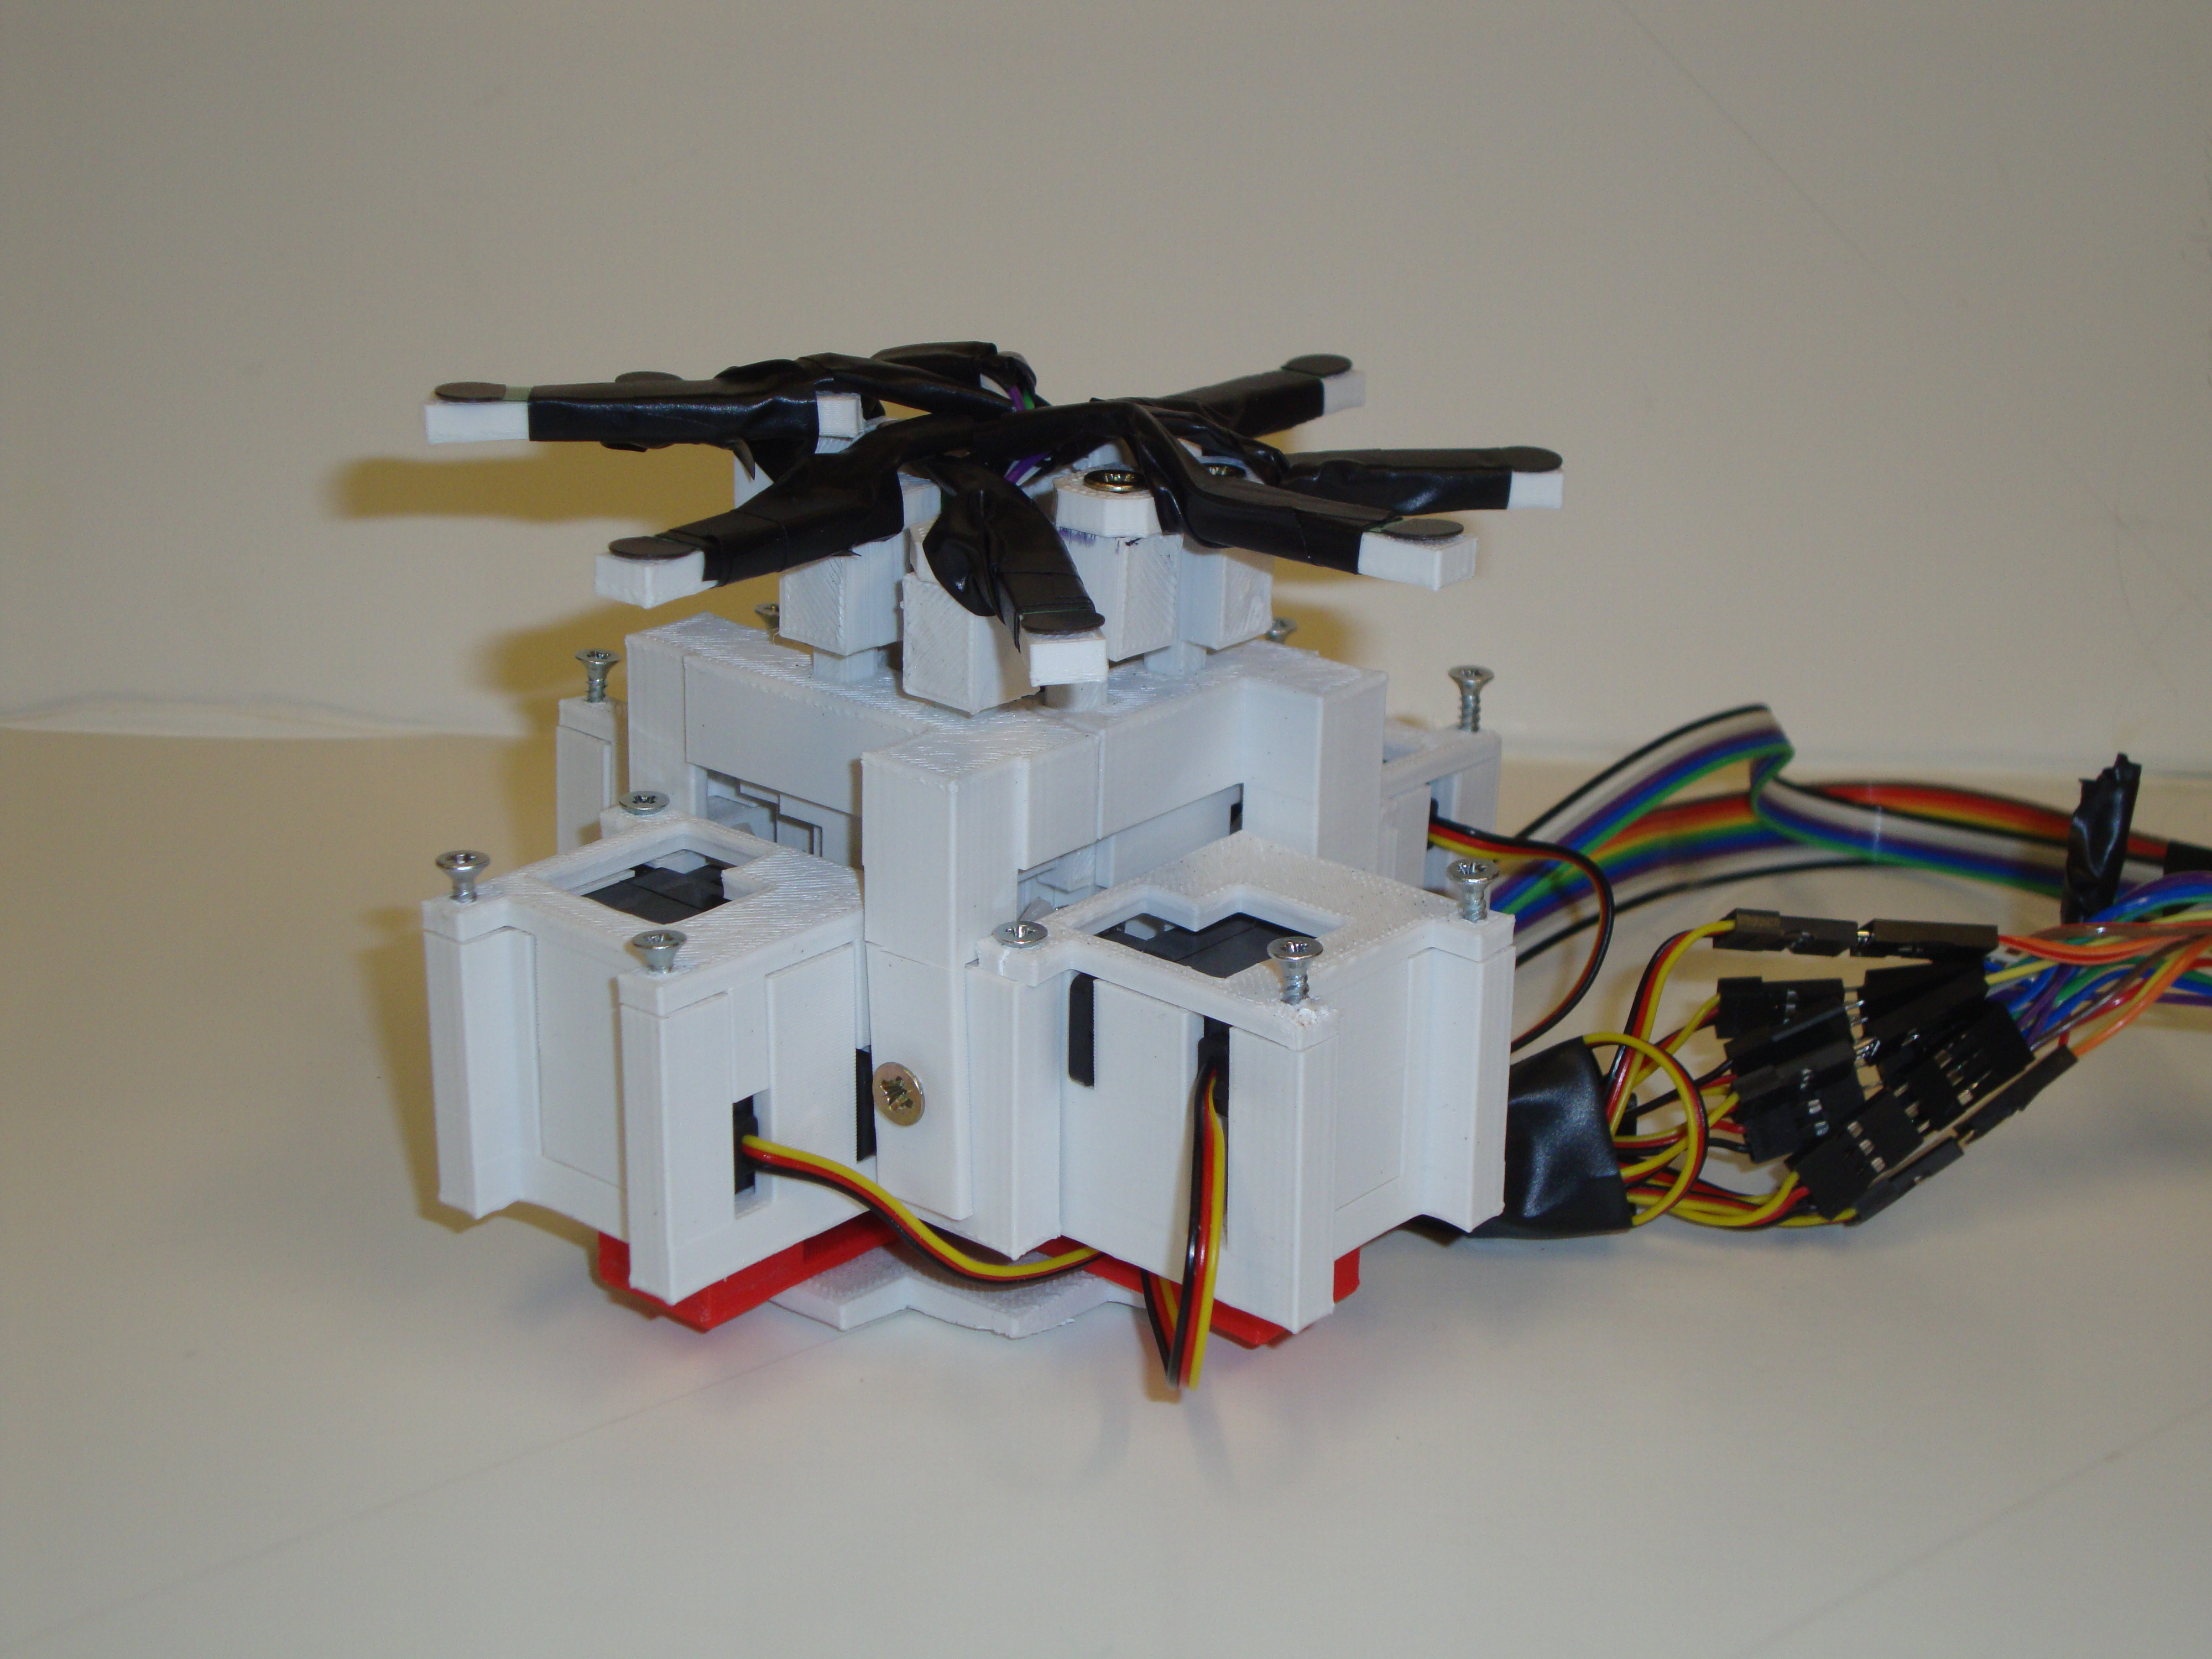
\includegraphics[width=0.7\textwidth]{HaptiQ1.JPG}
  \caption{8-HaptiQ}
  \label{fig:8-HaptiQ}
\end{figure}

The 4-HaptiQ not only is not optimised in terms of space, but its wiring is also not well engineered. As it is possible to observe in figure ~\ref{fig:HaptiQ reference static actuators} the wiring does not allow the device to be used comfortably, especially when one wants to rotate it. 

\section{The API}

\begin{itemize}
	\item explain the API structure
    \item see notes below
\end{itemize}

\section{Tactons}


\section{Applications}

\section{NOTES:}

 The HTP provides the following properties through a single point haptic cue \todo[noline]{this paragraph is partially copied from paper} :
\begin{itemize}
\item \textbf{EMPHASIS ON THE DESIGN CHOICES OF HAPTIQ, like not having a break or not doing any texture behaviours}
	\item height and texture: "the relief and tactile feel that corresponds to elements displayed on the table".
    \item malleability: "how different materials respond to touch and pressure".
    \item friction: "resistance to movement in directions parallel to the table plane".
    \item location: "different positions on the table should provide appropriate haptic feedback".
    \item multiplicity: "the ability to provide multi-user or multi-point haptic feedback simultaneously". \cite{marquardt2009haptic}
\end{itemize}



\begin{enumerate}
	\item Hardware design
    	\begin{enumerate}
        \item FIRST ITERATION
        	\item Improving the actuators
            	show pictures of old HTP and new MHTP
            \item pressure sensors (they are optional)
            \item actuators position facilitate directions. this is useful for blind people. an alternative device could provide actuators displaced as a grid.
            \item 4-MHTP
            \item 8-MHTP
            \item touch screen display SDK should be able to provide raw input
            \item from Brock's : "most blind seem to explore tactile maps with both hands and all 10 fingers"
            \item the computer needs a sound card for enabling text-to-speech output
        \end{enumerate}
	\item MHTP API architecture
    	\begin{enumerate}
        	\item state what architecture is targeted
        	\item Factory pattern with reflection in combination with delegation pattern was used to abstract the input from the touch screen device and notify the MHTP manager system
            \item Observer pattern is used to notify haptic shapes about any new input
            \item Bytetags (or glyphs?) were used to get input from touch screen device (Implementation?)
            \item custom configuration
            \item API allows recognition of glyphs using different devices (touch displayes via surface sdk, webcam, etc)
            \item Limitations: there is a lower bound threshold on how often input can be acquired. this depends on the input device, the input technique used and the "refresh rate" of the MHTP
            \item texture recognition not impemented because servos cannot act over a certain frequency. Papert \cite{brown2005first} has a part where it says what's the skin frequency range. Solutions could include electro-vibration or haptic vibration motors (http://www.precisionmicrodrives.com/vibrating-vibrator-vibration-motors)
        \end{enumerate}
    \item MHTP API allows both high and low level manipulation of the device (in a similar fashion to HTP toolkit)
    \item Behaviour design
    \item Haptic objects
    \item Text exploration using SpeechSynthetiser - this can be personalised by adding custom haptic shapes which can react differently
\end{enumerate}


\textbf{NOTES:}

\begin{itemize}
    \item Ungar's paper --> conjoint retention hypothesis: combining spatial and linguistic information
    \item Ungar's paper --> "overall performance increases because the dual perceptual/linguistic representation provides a richer cueing and retrieval base for the learner to draw from during recall"
    \item Ungar's paper does not show any strong evidence that linguistic representation might add more to the perceptual one. However, that's a study from 2001
    \item MHTP can be classified as TUI but dynamic (see Ullmer 2005)
\end{itemize}

